% Descripción de estos servidores 
Un servidor web es un programa que utiliza el protocolo de transferencia de hipertexto HTTP, para servir los archivos que forman páginas web a los usuarios, en respuesta a sus solicitudes. Esos archivos son reenviados por los clientes HTTP de las computadoras de los usuarios . Las comptadoras y los dispositivos dedicados también pueden denominarse servidores Web.
\subsubsection{Instalación del servidor}
Utilizamos el servidor Apache2 como nuestro servidor HTTP. Los pasos para su instalación son los siguientes:
\begin{figure}[!htbp]
	\hypertarget{fig:instalacionHTTP}{\hspace{1pt}}
	\begin{center}
		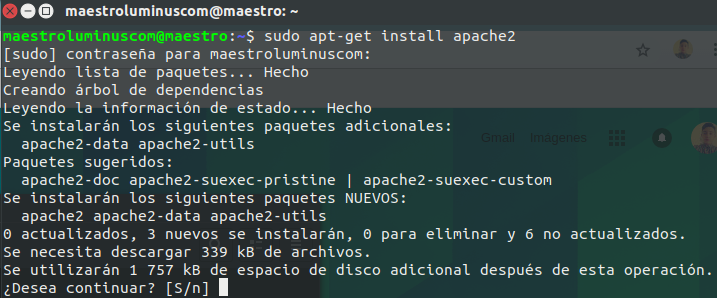
\includegraphics[width=0.7\textwidth]{desarrollo/tarea2/img/instalacionHTTP.png}
		\caption{Instalación del servidor.}
		\label{fig:instalacionHTTP}
	\end{center}
\end{figure}
\subsubsection{Sensor}
Este sensor está escrito en Bash. Toma como datos de entrada el servidor al que se le va a hacer la petición y la petición que se le va a hacer.
\begin{figure}[!htbp]
	\hypertarget{fig:sensorHTTP}{\hspace{1pt}}
	\begin{center}
		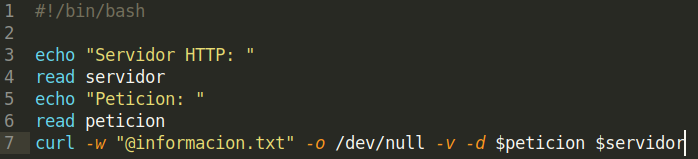
\includegraphics[width=0.7\textwidth]{desarrollo/tarea2/img/sensorHTTP.png}
		\caption{Código del sensor HTTP.}
		\label{fig:sensorHTTP}
	\end{center}
\end{figure}
\pagebreak
\begin{figure}[!htbp]
	\hypertarget{fig:outputHTTP}{\hspace{1pt}}
	\begin{center}
		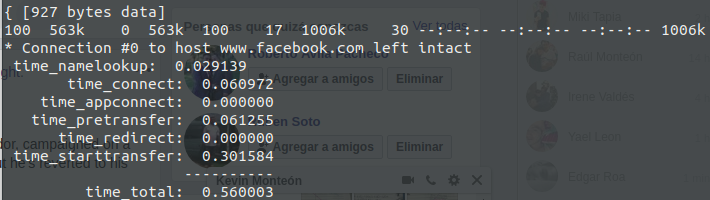
\includegraphics[width=0.7\textwidth]{desarrollo/tarea2/img/outputHTTP.png}
		\caption{Datos de salida del sensor HTTP.}
		\label{fig:outputHTTP}
	\end{center}
\end{figure}